\documentclass[11pt,a4paper]{article}

\usepackage[margin=1in]{geometry}
\usepackage[hidelinks]{hyperref}
\usepackage{amsmath}
\usepackage{enumitem}
\usepackage{booktabs}
\usepackage{longtable}
\usepackage{xcolor}
\usepackage{listings}
\usepackage{tikz}
\usetikzlibrary{arrows.meta, positioning, shapes.geometric}

\definecolor{codebg}{HTML}{F5F5F5}
\definecolor{codecomment}{HTML}{5C6B73}
\definecolor{codekey}{HTML}{0F4C75}
\definecolor{codestr}{HTML}{B8336A}

\lstdefinestyle{plain}{
  backgroundcolor=\color{codebg},
  basicstyle=\ttfamily\footnotesize,
  commentstyle=\color{codecomment},
  keywordstyle=\color{codekey}\bfseries,
  stringstyle=\color{codestr},
  showstringspaces=false,
  breaklines=true,
  frame=single,
  framesep=4pt,
  framerule=0pt,
  xleftmargin=6pt,
  xrightmargin=6pt
}
\lstset{style=plain}

\title{\textbf{MovieSentiment --- Project Workflow}\\[2pt]
       \large End-to-End MLOps Pipeline for IMDb Sentiment Analysis}
\author{Soumya Sarkar}
\date{\today}

\begin{document}

\maketitle

\begin{abstract}
\noindent MovieSentiment is a production-grade MLOps demonstrator that ingests IMDb
movie reviews, trains both a classical baseline and a fine-tuned transformer, exports
the transformer to a quantised ONNX runtime, serves predictions through a FastAPI
service deployed on AWS ECS Fargate, and closes the loop with drift detection that
triggers automated weekly retraining. This document walks through every stage of that
pipeline in order, describes the design choices behind it, and points at the file in
the repository where each piece lives so a reader can follow the code along with the
prose.
\end{abstract}

\tableofcontents
\newpage

% ----------------------------------------------------------------------------
\section{High-Level Architecture}
% ----------------------------------------------------------------------------

The project follows a familiar but tightly engineered loop: \emph{data} flows into
\emph{training}, which produces a versioned \emph{model artefact}, which is loaded by
the \emph{serving} layer, whose live traffic is observed by the \emph{monitoring}
layer, which in turn can fire the training loop again.

\begin{center}
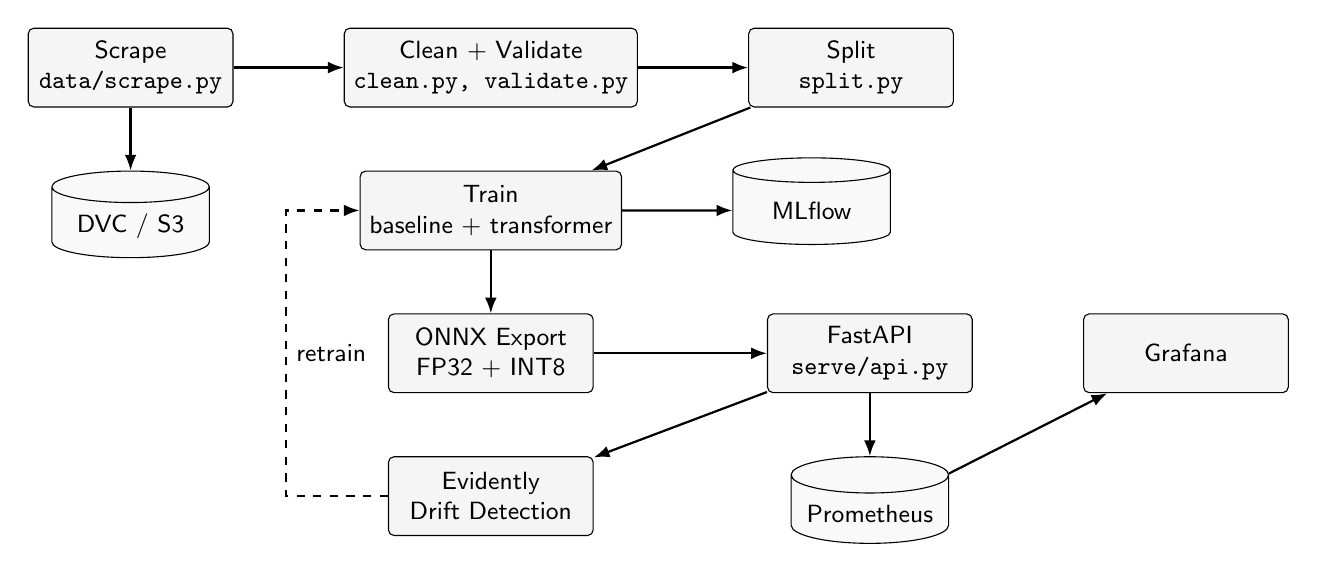
\begin{tikzpicture}[
  node distance=8mm and 14mm,
  every node/.style={font=\small\sffamily},
  box/.style={draw, rounded corners=2pt, align=center, minimum width=26mm,
              minimum height=10mm, fill=gray!8},
  store/.style={draw, cylinder, shape border rotate=90, aspect=0.25,
                minimum width=20mm, minimum height=11mm, fill=gray!5},
  arrow/.style={-{Latex[length=2mm]}, thick}
]

\node[box]   (scrape) {Scrape \\ \texttt{data/scrape.py}};
\node[box, right=of scrape] (clean)  {Clean + Validate \\ \texttt{clean.py, validate.py}};
\node[box, right=of clean]  (split)  {Split \\ \texttt{split.py}};
\node[store, below=of scrape] (dvcs3) {DVC / S3};

\node[box, below=of clean]  (train)  {Train \\ baseline + transformer};
\node[store, right=of train] (mlflow) {MLflow};
\node[box, below=of train]  (onnx)   {ONNX Export \\ FP32 + INT8};

\node[box, right=of onnx, xshift=8mm] (api) {FastAPI \\ \texttt{serve/api.py}};
\node[store, below=of api]  (prom) {Prometheus};
\node[box, right=of api]    (grafana) {Grafana};
\node[box, below=of onnx]   (drift) {Evidently \\ Drift Detection};

\draw[arrow] (scrape) -- (clean);
\draw[arrow] (clean)  -- (split);
\draw[arrow] (scrape) -- (dvcs3);
\draw[arrow] (split)  -- (train);
\draw[arrow] (train)  -- (mlflow);
\draw[arrow] (train)  -- (onnx);
\draw[arrow] (onnx)   -- (api);
\draw[arrow] (api)    -- (prom);
\draw[arrow] (prom)   -- (grafana);
\draw[arrow] (api)    -- (drift);
\draw[arrow, dashed] (drift) -- ++(-2.6,0) |- node[pos=0.25, right] {retrain} (train);

\end{tikzpicture}
\end{center}

\noindent The dashed line in the diagram is the closed-loop feedback: when Evidently
reports that the production input distribution has drifted past 30\% of features,
the drift workflow dispatches the weekly retrain workflow and the cycle starts again.

% ----------------------------------------------------------------------------
\section{Repository Layout}
% ----------------------------------------------------------------------------

A reader who clones the repository will find the following top-level folders.

\begin{longtable}{@{}lp{0.65\linewidth}@{}}
\toprule
\textbf{Path} & \textbf{Purpose} \\
\midrule \endhead
\texttt{src/moviesentiment/}    & The installable Python package. All pipeline logic lives here. \\
\texttt{src/.../data/}          & Scrape, clean, split, validate. \\
\texttt{src/.../models/}        & Baseline, transformer, ONNX export, registry helpers. \\
\texttt{src/.../serve/}         & FastAPI app, inference engine, async router, explain, tracing, logging. \\
\texttt{src/.../monitor/}       & Prometheus metrics, Evidently drift, NannyML performance estimation. \\
\texttt{src/.../eval/}          & Confusion matrix, ROC/PR, calibration, slice analysis. \\
\texttt{src/.../cli.py}         & Typer CLI -- the single entry point for every stage. \\
\texttt{src/.../config.py}      & Pydantic settings (env-var driven, prefix \texttt{MS\_}). \\
\texttt{tests/}                 & pytest suite, including hypothesis property tests. \\
\texttt{deploy/}                & Dockerfile, docker-compose, ECS task definition, Lambda handler, Grafana, Prometheus. \\
\texttt{scripts/}               & SageMaker launcher, Locust load test, lock-file compiler, train entrypoint. \\
\texttt{frontend/}              & Single-page static demo UI. \\
\texttt{docs/}                  & Model card, datasheet, benchmarks, drift reports, future improvements, this file. \\
\texttt{.github/workflows/}     & CI, retrain, drift, scrape, benchmark, scorecard. \\
\texttt{dvc.yaml}, \texttt{params.yaml} & The reproducible pipeline definition + hyperparameters. \\
\texttt{Makefile}               & Thin wrappers that the developer calls day to day. \\
\bottomrule
\end{longtable}

% ----------------------------------------------------------------------------
\section{Data Pipeline}
% ----------------------------------------------------------------------------

\subsection{Scraping (\texttt{src/.../data/scrape.py})}

Two ingestion paths are wired in. The default path, \texttt{source=hf}, downloads the
\texttt{stanfordnlp/imdb} dataset from HuggingFace (50{,}000 labelled reviews).
The dataset revision is pinned through the \texttt{MS\_HF\_REVISION} environment
variable, which is checked into the security model so that a namespace takeover on
HuggingFace cannot inject malicious data into a training run. The alternative path,
\texttt{source=live}, performs a paginated GraphQL scrape against IMDb's persisted
query endpoint and emits the same canonical schema; in practice IMDb sits behind AWS
WAF, so the live path is documented but not used in CI.

Every record written to \texttt{data/raw/reviews.parquet} has the schema
\texttt{(review\_id, movie\_id, text, rating, scraped\_at, label)}. The output file is
tracked by DVC and pushed to an S3 remote (\texttt{moviesentiment-dvc-soumya}).

\subsection{Cleaning (\texttt{src/.../data/clean.py})}

The cleaner strips HTML tags and URLs, lower-cases the text, collapses runs of
whitespace, drops null and ultra-short reviews (length $\leq 10$), and removes exact
duplicates. The output (\texttt{data/interim/clean.parquet}) is again tracked by DVC.

\subsection{Data Validation (\texttt{src/.../data/validate.py})}

The validation stage is a deliberate ``halt the pipeline'' gate. Six expectations are
checked against the cleaned dataset:

\begin{itemize}[leftmargin=*]
\item \textbf{schema}: columns must contain \texttt{\{text, label\}}.
\item \textbf{no\_null\_text}, \textbf{no\_null\_label}.
\item \textbf{text\_length}: $10 \leq \text{len}(\text{text}) \leq 5000$.
\item \textbf{label\_values}: \texttt{label} $\in \{0, 1\}$.
\item \textbf{label\_balance}: $0.40 \leq P(\text{label}=1) \leq 0.60$.
\end{itemize}

Any failure produces a non-zero exit code, which propagates up through DVC so
\texttt{dvc repro} aborts before training starts. The report is written to
\texttt{metrics/data\_quality.json} as a non-cached metric, so DVC always inspects
the latest report rather than restoring an old one from the cache.

\subsection{Splitting (\texttt{src/.../data/split.py})}

The cleaned dataset is split into \texttt{train/val/test} with stratification on the
\texttt{label} column. Sizes are read from \texttt{params.yaml} (default
\texttt{test\_size=0.15}, \texttt{val\_size=0.15}, \texttt{seed=42}). Because
\texttt{val\_size} is given relative to the full dataset, the splitter adjusts it
when applied to the trainval subset so the final split matches the requested ratios.

\subsection{DVC Pipeline (\texttt{dvc.yaml})}

All four data stages plus the two training stages are declared in \texttt{dvc.yaml},
with their inputs, outputs, params, and metrics. Running \texttt{dvc repro} from the
repository root walks the DAG and reruns only the stages whose deps have changed.

\begin{lstlisting}[language=Python, caption={Pipeline DAG (simplified from \texttt{dvc.yaml})}]
scrape -> clean -> validate_data -> split -> train_baseline
                                         -> train_transformer
\end{lstlisting}

% ----------------------------------------------------------------------------
\section{Training}
% ----------------------------------------------------------------------------

\subsection{Baseline (\texttt{src/.../models/baseline.py})}

The baseline is a scikit-learn \texttt{Pipeline} of \texttt{TfidfVectorizer} (1--2
grams, 50{,}000 features, sublinear TF) and \texttt{LogisticRegression}
($C=1.0$, class-balanced, $\text{max\_iter}=1000$). The trained pipeline is dumped
to \texttt{models/baseline.joblib} and logged to MLflow with parameters, three
metrics (\texttt{accuracy}, \texttt{macro\_f1}, \texttt{roc\_auc}), and a confusion
matrix artifact. The same metrics are written to \texttt{metrics/baseline.json} so
the DVC stage can track them.

\subsection{Transformer (\texttt{src/.../models/transformer.py})}

The transformer is a \texttt{distilbert-base-uncased} fine-tune driven by the
HuggingFace \texttt{Trainer}. Key behaviours:

\begin{itemize}[leftmargin=*]
\item \textbf{Tokenisation} is batched and lazy via \texttt{datasets.Dataset.map}.
\item \textbf{Revision pinning}: \texttt{from\_pretrained} receives an explicit
      \texttt{revision} arg sourced from \texttt{params.yaml} or the
      \texttt{MS\_HF\_REVISION} env var. This blocks namespace-takeover attacks.
\item \textbf{LoRA} (\texttt{peft}) is opt-in via \texttt{params.yaml::transformer.use\_lora}.
      Rank-8 adapters target \texttt{q\_lin} and \texttt{v\_lin} in DistilBERT's
      attention layers, which means training $\sim$0.3\% of the parameters and
      writing a $\sim$3\,MB adapter on top of the 250\,MB frozen base. This is the
      mode that the drift-triggered retrain uses.
\item \textbf{Mixed precision} (\texttt{fp16}) is enabled when CUDA is visible.
\item \textbf{Evaluation} happens every epoch; the best checkpoint by macro-F1 is
      loaded back at the end.
\item \textbf{Logging}: parameters, metrics, classification report, ROC, PR,
      calibration, and confusion matrix all land in MLflow. The trained model is
      logged via \texttt{mlflow.transformers.log\_model} and registered under the
      configured \texttt{model\_name} (\texttt{moviesentiment-classifier}).
\end{itemize}

\subsection{MLflow Tracking and Registry}

The default tracking URI is \texttt{sqlite:///mlflow.db} so the entire pipeline can
run on a laptop. A production deployment is documented in the README as ``replace the
SQLite backend with managed Postgres + S3 artifact store''. Models are promoted to
the \texttt{Production} stage; the inference engine reads
\texttt{settings.model\_stage} when bootstrapping.

\subsection{SageMaker Launcher (\texttt{scripts/sagemaker\_launch.py})}

For the rare full fine-tune the project uses SageMaker on \texttt{ml.g4dn.xlarge}
(T4 GPU, $\sim$\$0.30 per run). Spot training is enabled by default, with
\texttt{max\_wait = 2 * max\_run} and a checkpoint S3 URI so SageMaker can pause
and resume on spot interruption. The launcher stages a minimal source directory into
a temp folder (the repo itself is too large to tar verbatim) and submits the
\texttt{PyTorch} estimator.

% ----------------------------------------------------------------------------
\section{ONNX Export and Quantisation}
% ----------------------------------------------------------------------------

The serving runtime is \emph{not} PyTorch. The fine-tuned DistilBERT is exported to
ONNX and then quantised to INT8 weights so it can run on a 0.25 vCPU Fargate task
in single-digit milliseconds. The export pipeline lives in
\texttt{src/.../models/onnx\_export.py} and runs four steps:

\begin{enumerate}[leftmargin=*]
\item \textbf{Locate source.} \texttt{models/distilbert/} if it exists; otherwise
      fall back to \texttt{distilbert-base-uncased}.
\item \textbf{Export.} \texttt{ORTModelForSequenceClassification.from\_pretrained(...,
      export=True)} writes \texttt{model.onnx} into
      \texttt{models/distilbert\_onnx/}.
\item \textbf{Quantise.} \texttt{onnxruntime.quantization.quantize\_dynamic} produces
      \texttt{models/distilbert\_onnx\_int8/model.onnx} with QInt8 weights.
\item \textbf{Benchmark.} 5 warmup runs + 100 timed runs on a batch of 2 sentences at
      \texttt{max\_length=128}. Mean, p50, p95, and p99 latencies for both FP32 and
      INT8 are written to \texttt{docs/benchmarks.md} and
      \texttt{metrics/onnx\_benchmark.json}.
\end{enumerate}

Both ONNX artefacts are DVC-tracked
(\texttt{models/distilbert\_onnx.dvc}, \texttt{...\_int8.dvc}). The serving container
bundles only the ONNX artefacts -- never the raw HuggingFace checkpoints.

\begin{longtable}{@{}lrrrrr@{}}
\toprule
\textbf{Model} & \textbf{Accuracy} & \textbf{Macro F1} & \textbf{ROC-AUC} &
\textbf{p50 CPU} & \textbf{Size} \\
\midrule
TF-IDF + LR          & 0.904 & 0.904 & 0.967 & $<5$ ms & 18 MB  \\
DistilBERT FP32 ONNX & 0.939 & 0.939 & 0.984 & 14.1 ms & 256 MB \\
DistilBERT INT8 ONNX & 0.939 & 0.939 & 0.984 & 6.8 ms  & 64 MB  \\
\bottomrule
\end{longtable}

% ----------------------------------------------------------------------------
\section{Serving Layer}
% ----------------------------------------------------------------------------

\subsection{FastAPI Application (\texttt{src/.../serve/api.py})}

The serving app is a single FastAPI application whose lifespan handler loads the
ONNX-INT8 model into an \texttt{InferenceEngine} once at startup and keeps the
session warm. The app exposes the following routes:

\begin{longtable}{@{}lp{0.62\linewidth}@{}}
\toprule
\textbf{Endpoint} & \textbf{Behaviour} \\ \midrule \endhead
\texttt{GET /healthz}   & Liveness probe; always 200 once the process is up. \\
\texttt{GET /readyz}    & Readiness probe; 503 until the engine is ready. \\
\texttt{GET /version}   & Reports \texttt{model\_name}, \texttt{model\_stage},
                          and the git SHA baked into the image. \\
\texttt{GET /metrics}   & Prometheus exposition (default + custom metrics). \\
\texttt{GET /sample}    & Reservoir-sampler statistics for debugging. \\
\texttt{POST /predict}  & Synchronous batch inference; max batch 32, rate-limited
                          to 60/minute per IP. \\
\texttt{POST /explain}  & Per-token attribution via occlusion;
                          rate-limited to 10/minute per IP. \\
\texttt{POST /predict/async} & Submit a batch to SQS for the Lambda worker;
                               503 if AWS infra is not configured. \\
\texttt{GET /predict/result/\{id\}} & Read async-job state from DynamoDB. \\
\texttt{GET /ui/}       & Static frontend (if \texttt{frontend/index.html} is bundled). \\
\bottomrule
\end{longtable}

\subsection{Inference Engine (\texttt{src/.../serve/inference.py})}

The engine wraps an \texttt{onnxruntime.InferenceSession} with
\texttt{CPUExecutionProvider}. INT8 is preferred; FP32 is used as a fallback. The
tokenizer is loaded from the same directory as the ONNX file, which is always a
local DVC-pulled path -- never a remote HuggingFace identifier at serve time.
Predictions are computed in pure NumPy: softmax, argmax, confidence. The label
mapping is \texttt{0$\rightarrow$negative}, \texttt{1$\rightarrow$positive}.

\subsection{Input Validation (\texttt{src/.../serve/schemas.py})}

All request and response bodies are Pydantic models with strict bounds:

\begin{itemize}[leftmargin=*]
\item \texttt{PredictRequest.texts}: \texttt{min\_length=1}, \texttt{max\_length=32}.
\item \texttt{ExplainRequest.text}: \texttt{min\_length=1}, \texttt{max\_length=5000};
      \texttt{top\_k}: $1 \leq k \leq 50$.
\item Per-text length is checked against \texttt{settings.max\_text\_length}
      ($5000$) in the route itself, on top of the schema.
\end{itemize}

\subsection{Reservoir Sampling (\texttt{src/.../serve/reservoir.py})}

Production inputs feed the drift detector, but capturing 100\% of traffic is
prohibitively expensive and a naive 10\% sample biases toward early traffic. The
serving layer therefore uses Vitter's Algorithm R reservoir sampler at $k=1000$
under a thread lock. After $n$ items every input has identical probability $k/n$ of
being retained, independent of arrival order. The reservoir is flushed to
\texttt{data/production/recent.parquet} every 100 inserts. The sampler's statistics
are exposed at \texttt{GET /sample} for debugging.

\subsection{Occlusion-Based Explanations (\texttt{src/.../serve/explain.py})}

\texttt{POST /explain} produces per-token attribution by dropping each whitespace
token one at a time, re-running inference on the resulting batch, and reporting the
delta in the predicted-class probability. If a drop flips the predicted label, the
attribution is the sum of both confidences -- a clear signal that the token was
load-bearing. Top-$k$ tokens (default 10) are returned. The cost is $\mathcal{O}(K)$
inference calls per request, which is why \texttt{/explain} sits behind a much
tighter rate limit than \texttt{/predict}.

\subsection{Async Path (\texttt{src/.../serve/async\_api.py},
                       \texttt{deploy/lambda/async\_predict\_handler.py})}

For batch jobs that would otherwise tie up Fargate threads, the project exposes an
async path:

\begin{enumerate}[leftmargin=*]
\item \texttt{POST /predict/async} writes a row to DynamoDB (\texttt{status=queued})
      and publishes the \texttt{job\_id} to SQS.
\item The SQS event source mapping fires the Lambda. The handler downloads the ONNX
      model from S3 into \texttt{/tmp} (cached across warm invocations), tokenises,
      runs inference, and updates DynamoDB with \texttt{status=complete} and the
      predictions.
\item \texttt{GET /predict/result/\{job\_id\}} reads DynamoDB.
\end{enumerate}

If \texttt{MS\_SQS\_QUEUE\_URL} or \texttt{MS\_JOBS\_TABLE} are unset, the router
still mounts and every call returns 503, so local development works without any
AWS plumbing.

\subsection{Structured Logging (\texttt{src/.../serve/logging\_setup.py})}

\texttt{structlog} is configured with a JSON renderer and a contextvars-based
request-id binding. A FastAPI middleware reads the inbound \texttt{x-request-id}
header (or mints one if missing) and binds it to the context so every log line
emitted by the request carries the same identifier. The id is also written back on
the response so callers can correlate. Inbound ids are sanitised against the regex
\texttt{[A-Za-z0-9.\_-]} and capped at 64 characters, which closes the CRLF
log-injection vector and bounds the maximum size a hostile client can grow log
lines to.

\subsection{Tracing (\texttt{src/.../serve/tracing.py})}

OpenTelemetry tracing is opt-in. If \texttt{OTEL\_EXPORTER\_OTLP\_ENDPOINT} is set,
the app wires an \texttt{OTLPSpanExporter} into a \texttt{TracerProvider} and
instruments FastAPI through \texttt{FastAPIInstrumentor}. The intended target is
Grafana Cloud's free tier (50\,GB traces forever). When the env var is unset, the
function returns immediately, so the production no-op cost is zero.

\subsection{Rate Limiting and CORS}

\texttt{slowapi} provides per-IP rate limits on \texttt{/predict} (60/min) and
\texttt{/explain} (10/min). The CORS middleware reads
\texttt{MS\_CORS\_ALLOW\_ORIGINS} (comma-separated list). The default is the
wildcard \texttt{*} without credentials, which is the only configuration browsers
accept; setting any explicit allowlist automatically enables credentials.

\subsection{Custom Prometheus Metrics (\texttt{src/.../monitor/prometheus.py})}

On top of the default HTTP histograms from
\texttt{prometheus-fastapi-instrumentator}, the project exposes:

\begin{itemize}[leftmargin=*]
\item \texttt{prediction\_confidence} (Histogram, buckets at 0.5, 0.6, 0.7, 0.8,
      0.9, 0.95, 0.99, 1.0).
\item \texttt{prediction\_class\_total} (Counter, label = \texttt{label}).
\item \texttt{model\_version\_info} (Gauge, labels = \texttt{model\_name},
      \texttt{version}, \texttt{git\_sha}) -- set once at startup.
\item \texttt{model\_estimated\_f1} (Gauge, label = \texttt{metric}) -- set by the
      NannyML estimator.
\end{itemize}

% ----------------------------------------------------------------------------
\section{Monitoring and Drift}
% ----------------------------------------------------------------------------

\subsection{Evidently Drift Reports (\texttt{src/.../monitor/drift.py})}

\texttt{run\_drift\_report} builds an Evidently \texttt{DataDriftPreset} report
comparing the training distribution (\texttt{data/processed/train.parquet}) to the
sampled production stream (\texttt{data/production/recent.parquet}). Two derived
text features are added before the comparison: \texttt{text\_length} and
\texttt{word\_count}. The report is written as HTML into
\texttt{docs/drift\_reports/<date>.html}. A lighter helper, \texttt{drift\_share},
returns just the share of drifted columns as a float so CI workflows can branch on
it without parsing HTML.

\subsection{NannyML Performance Estimation (\texttt{src/.../monitor/perf\_estimate.py})}

Drift on the inputs does not necessarily mean the model is wrong on the new
distribution. NannyML's Confidence-Based Performance Estimation (CBPE) uses the
production prediction confidences plus calibration learnt on a labelled reference
set to estimate F1 and ROC-AUC \emph{without} requiring ground-truth labels for the
production data. The estimator emits the result on the \texttt{model\_estimated\_f1}
gauge, so the same Grafana dashboard that shows drift also shows
expected-performance-under-drift.

\subsection{Local Observability Stack (\texttt{deploy/docker-compose.yml})}

The local \texttt{docker compose} bundles three services: the API itself,
Prometheus (with a 7-day retention), and Grafana with anonymous Admin access and a
pre-provisioned dashboard.

% ----------------------------------------------------------------------------
\section{Frontend}
% ----------------------------------------------------------------------------

\texttt{frontend/index.html} is a single, self-contained HTML file with a
terminal-monochrome aesthetic (accent \texttt{\#00ff88}). It implements a
three-mode demo:

\begin{itemize}[leftmargin=*]
\item \textbf{mock}: a JavaScript keyword classifier so the UI works without an
      API at all (GitHub Pages friendly).
\item \textbf{auto}: fetches the current ECS Fargate public IP from a stored
      \texttt{api.json}.
\item \textbf{custom}: lets the visitor paste an IP and call their own deployment.
\end{itemize}

\noindent The page also renders an animated SVG architecture flow and a live
activity strip. It is served two ways: as a static site on GitHub Pages \emph{and}
from \texttt{/ui/} on the Fargate task itself -- when \texttt{frontend/index.html}
is present, the API mounts it via \texttt{fastapi.staticfiles.StaticFiles}. Cost on
AWS is unchanged because it is bundled into the same image.

% ----------------------------------------------------------------------------
\section{Containerisation and Deployment}
% ----------------------------------------------------------------------------

\subsection{Dockerfile}

A two-stage build:

\begin{enumerate}[leftmargin=*]
\item \textbf{builder}: \texttt{python:3.11-slim}, installs \texttt{uv}, then
      \texttt{uv pip install --system --no-cache ".[train]"} followed by
      \texttt{uv pip install --system --no-cache .}.
\item \textbf{runtime}: \texttt{python:3.11-slim}; copies the site-packages and
      \texttt{uvicorn} binary from the builder, copies \texttt{src/},
      \texttt{frontend/}, and only the two ONNX model directories. Runs as a
      non-root user \texttt{app} (uid 1000). \texttt{GIT\_SHA} is a build arg so
      \texttt{/version} can report the deployed commit. Healthcheck pings
      \texttt{/healthz} every 30 seconds.
\end{enumerate}

\subsection{ECS Task Definition (\texttt{deploy/ecs-task-definition.json})}

The task runs on \textbf{Fargate ARM64 Graviton} at \texttt{0.25 vCPU} and
\texttt{1024 MB} -- the smallest possible Fargate footprint, which is the entire
point of the INT8 quantisation. The image lives in ECR, logs stream to
CloudWatch (\texttt{/ecs/moviesentiment}), and the container healthcheck hits
\texttt{/healthz}. Environment variables: \texttt{OTEL\_SERVICE\_NAME},
\texttt{MS\_ENV=prod}, \texttt{PORT=8000}.

Monthly cost target: $\sim$\$6/mo on Graviton + a negligible amount of egress.

\subsection{CI-Driven Deploy}

The CI workflow (\texttt{.github/workflows/ci.yml}) does the deploy too. On
\texttt{push} to \texttt{main}, after the lint/test/security pass, the
\texttt{build-image} job:

\begin{itemize}[leftmargin=*]
\item Pulls the DVC-tracked ONNX artefacts from S3 (using \texttt{AWS\_ACCESS\_KEY\_ID}
      and \texttt{AWS\_SECRET\_ACCESS\_KEY} secrets).
\item Logs into GHCR \emph{and} ECR.
\item Sets up QEMU + Buildx for \texttt{linux/arm64}.
\item Builds the image with \texttt{GIT\_SHA=\$\{\{ github.sha \}\}} and pushes it to
      both registries under tags \texttt{:<sha>} and \texttt{:latest}.
\item Calls \texttt{aws ecs update-service --force-new-deployment} so Fargate rolls
      to the new image.
\end{itemize}

% ----------------------------------------------------------------------------
\section{CI/CD Workflows}
% ----------------------------------------------------------------------------

\begin{longtable}{@{}lp{0.62\linewidth}@{}}
\toprule
\textbf{Workflow} & \textbf{Trigger \& purpose} \\ \midrule \endhead
\texttt{ci.yml} & On every push + PR. Runs ruff, black, mypy on \texttt{src tests},
                  bandit, pip-audit (with documented \texttt{--ignore-vuln} list),
                  pytest with a coverage floor of 75\%, then builds the ARM64 image
                  and force-deploys to ECS on main. \\
\texttt{train.yml} & Weekly cron (Mon 02:00 UTC) plus manual dispatch. Pulls
                     processed data, retrains the baseline, compares macro-F1 to the
                     stored production value, and only chains the deploy job if the
                     model improved by $\geq 0.5\%$ (or \texttt{force\_promote} is
                     true). \\
\texttt{drift.yml} & Weekly cron (Mon 03:00 UTC), one hour after retrain. Pulls
                     the training data and production sample, runs
                     \texttt{drift\_share}, writes the HTML report, and calls
                     \texttt{train.yml} when the share exceeds 0.3. \\
\texttt{scrape.yml} & Weekly cron (Sun 00:00 UTC). Refreshes the raw HuggingFace
                      dataset and pushes the new pointer through DVC. \\
\texttt{weekly\_bench.yml} & Weekly cron (Mon 07:00 UTC). Pulls the ONNX artefact,
                             runs the latency benchmark, executes the slow
                             ONNX-export tests, and uploads \texttt{bench.txt} as
                             an artifact. \\
\texttt{scorecard.yml} & OSSF Scorecard supply-chain security analysis, weekly +
                         on branch protection rule changes. Uploads SARIF to
                         GitHub's code scanning. \\
\bottomrule
\end{longtable}

\noindent Dependabot (\texttt{.github/dependabot.yml}) opens weekly grouped PRs for
pip, GitHub Actions, and Docker base images.

% ----------------------------------------------------------------------------
\section{Security Posture}
% ----------------------------------------------------------------------------

The threat model and accepted residual risks live in \texttt{SECURITY.md}; the
short version is summarised here.

\begin{longtable}{@{}p{0.32\linewidth}p{0.6\linewidth}@{}}
\toprule
\textbf{Threat} & \textbf{Mitigation} \\ \midrule \endhead
Untrusted input $\to$ crash / RCE & Pydantic schema bounds; per-text length cap;
                                    ONNX-only inference (no \texttt{eval}, no
                                    \texttt{pickle}, no \texttt{exec}). \\
Traffic flood / DoS  & \texttt{slowapi} per-IP rate limits on \texttt{/predict}
                       (60/min) and \texttt{/explain} (10/min). \\
Log injection via headers & \texttt{x-request-id} allowlisted to
                            \texttt{[A-Za-z0-9.\_-]\{,64\}}; CRLF and control
                            chars stripped. \\
HF namespace takeover & \texttt{MS\_HF\_REVISION} pins an exact commit on every
                        \texttt{from\_pretrained} touching the Hub; serving only
                        loads local DVC-pulled artefacts. \\
Supply-chain (deps) & pip-audit + bandit on every PR; Dependabot weekly;
                      OSSF Scorecard weekly. \\
CORS abuse & Default \texttt{*} origin with \texttt{allow\_credentials=false}; an
             explicit allowlist auto-enables credentials. \\
PII in logs & \texttt{predict\_complete} logs counts + labels only;
              review-body sampling lives in S3 with no public prefix. \\
Container escalation & Image runs as \texttt{app} (uid 1000), no root shell tools. \\
\bottomrule
\end{longtable}

\noindent A handful of CVEs (transformers 5.x compatibility, starlette pin under
fastapi, pyOpenSSL under dvc[s3]) are accepted as residual risks with concrete
justification in \texttt{SECURITY.md} and \texttt{--ignore-vuln} entries in CI.

% ----------------------------------------------------------------------------
\section{Testing Strategy}
% ----------------------------------------------------------------------------

The test suite (\texttt{tests/}) targets a coverage floor of 75\%:

\begin{itemize}[leftmargin=*]
\item \texttt{test\_api.py} -- TestClient-based integration tests for every route,
      including 503-without-model behaviour, batch validation, request-id
      round-trip, CORS preflight, and the sanitiser unit tests.
\item \texttt{test\_inference.py}, \texttt{test\_explain.py}, \texttt{test\_reservoir.py}
      -- unit coverage for the serving primitives.
\item \texttt{test\_clean.py}, \texttt{test\_clean\_hypothesis.py},
      \texttt{test\_validate.py}, \texttt{test\_split.py} -- data layer, with
      property-based tests (\texttt{hypothesis}) on the cleaner.
\item \texttt{test\_scrape.py}, \texttt{test\_drift.py}, \texttt{test\_onnx\_export.py}
      -- pipeline edges; the ONNX e2e test is marked \texttt{slow}.
\end{itemize}

\noindent The Locust load test (\texttt{scripts/load\_test.py}) is invoked through
\texttt{make loadtest}; reference numbers live in \texttt{docs/loadtest.md}.

% ----------------------------------------------------------------------------
\section{Putting It All Together --- End-to-End Flow}
% ----------------------------------------------------------------------------

A successful round-trip through the system, top to bottom, is:

\begin{enumerate}[leftmargin=*]
\item \texttt{dvc repro} -- scrape, clean, validate, split, train baseline, train
      transformer, with MLflow logging every step.
\item \texttt{make export-onnx} -- export the fine-tuned DistilBERT, quantise to
      INT8, benchmark.
\item \texttt{dvc add models/distilbert\_onnx\_int8/} -- track the ONNX artefacts,
      then \texttt{dvc push} to S3.
\item \texttt{git push} -- triggers \texttt{ci.yml}: ruff, black, mypy, bandit,
      pip-audit, pytest with the 85\% coverage gate, calibration regression gate.
\item On \texttt{main}: the same workflow pulls the DVC artefacts, builds the
      ARM64 image, pushes to ECR and GHCR, and force-deploys ECS.
\item Fargate boots a new task; the lifespan loads the INT8 ONNX model; the
      healthcheck hits \texttt{/healthz}; the ALB or NLB routes traffic in.
\item Live traffic to \texttt{/predict} is sampled into a reservoir; Prometheus
      scrapes \texttt{/metrics}; Grafana renders the dashboard; OTel spans flow
      to Grafana Cloud.
\item Sunday: \texttt{scrape.yml} refreshes the raw dataset. Monday 02:00:
      \texttt{train.yml} retrains. 03:00: \texttt{drift.yml} compares
      distributions and, if drifted, re-fires \texttt{train.yml}.
\item NannyML CBPE re-estimates F1 from confidences alone; the gauge feeds the
      same Grafana panel.
\end{enumerate}

The loop is closed, every artefact has an owner, and every step is reproducible
from the repository alone given the right secrets.

\end{document}
